\subsection{幂均值教师中心、advantage 与可认证估计}
\label{sec:proximal-teacher-center}

本小节继续采用前节的单教师 BPO：固定前缀和完整正支持 $q,T$，记 $\rho=T/q$、$0\le\kappa\le1$、$0<\eta<1$。冻结教师信号、教师中心和中心化 advantage 分别为
\begin{align}
 A_{\kappa,\eta}(a)&=\begin{cases}
 \log\rho_a,&\kappa=0,\\
 (\kappa\eta)^{-1}\log(1-\eta+\eta\rho_a^\kappa),&\kappa>0,
 \end{cases}\\
 K_{\kappa,\eta}&=-\sum_aq_a A_{\kappa,\eta}(a),\\
 B_{\kappa,\eta}(a)&=A_{\kappa,\eta}(a)+K_{\kappa,\eta},\qquad \E_qB=0.
 \label{eq:center-explicit-definition}
\end{align}
当前 $K$ 已经含有 $1/\eta$。若缓存原始信号中心 $\widetilde K=-\E_qf$，则 $\widetilde K=\eta K$，在 BPO 系数中只除以 $\eta$ 一次。

$B$ 是条件中心化的教师监督，不是跨 response 的组 advantage。$A$、$K$ 在本轮 inner 中冻结；学生反馈 $C_qU/\eta$ 随参数改变。

\subsubsection{完整展开、KL 端点与凸散度表示}

几何端点恢复
\begin{equation}
 K_{0,\eta}=\sum_aq_a\log(q_a/T_a)=\KL(q\Vert T).
\end{equation}
一般形状则为
\begin{equation}
 \boxed{K_{\kappa,\eta}
 =-\frac1{\kappa\eta}\sum_aq_a
 \log\left(1-\eta+\eta(T_a/q_a)^\kappa\right).}
 \label{eq:center-expanded-k}
\end{equation}
算术端点满足
\begin{equation}
 K_{1,\eta}=\eta^{-1}\KL\big(q\Vert(1-\eta)q+\eta T\big).
\end{equation}
一般 $\kappa$ 下，若 $m$ 是归一化幂均值 target、$Z=\sum_aq_ae^{f_a}$，则
\begin{equation}
 K_{\kappa,\eta}=\frac{\KL(q\Vert m)-\log Z}{\eta}.
\end{equation}
所以不能把它继续标为原 teacher KL。

然而 $K$ 本身是一个合法的凸 $f$-divergence。定义
\begin{equation}
 \phi_{\kappa,\eta}(x)=x-1-
 \frac{\log(1-\eta+\eta x^\kappa)}{\kappa\eta},\qquad x>0.
 \label{eq:center-convex-generator}
\end{equation}
它满足 $\phi(1)=\phi'(1)=0$，且
\begin{equation}
 \phi''(x)=
 \frac{x^{\kappa-2}[(1-\kappa)(1-\eta)+\eta x^\kappa]}
 {(1-\eta+\eta x^\kappa)^2}>0.
\end{equation}
因此 $\phi(x)\ge0$，再由 $\E_q(\rho-1)=0$，得到
\begin{equation}
 K_{\kappa,\eta}=\E_q\phi_{\kappa,\eta}(T/q).
\end{equation}
这个式子的标准 $f$-divergence 参照测度是 $q$，第一分布是 $T$；其生成函数包含 $\kappa,\eta$。几何极限为 $\phi_0(x)=x-1-\log x$。它与普通 KL 或前文 $D_\kappa$ 的关系由上述端点和极限决定，不能因其非负就把名称混用。

\subsubsection{中心的有界性、单调性与小步极限}

\begin{theorem}[教师中心的分布无关界]
\label{thm:center-bounds-monotonicity}
令 $0<\kappa\le1$、$0<\eta<1$，则
\begin{equation}
 0\le K_{\kappa,\eta}
 \le\min\left\{\KL(q\Vert T),\;
 c_{\kappa,\eta}\right\},\qquad
 c_{\kappa,\eta}=-\frac{\log(1-\eta)}{\kappa\eta}.
 \label{eq:center-uniform-cap}
\end{equation}
$K=0$ 当且仅当 $q=T$。固定 $q,T$ 时，$K$ 随 $\kappa$ 非增加、随 $\eta$ 非减少。对任意至少二元的词表，上界 $c_{\kappa,\eta}$ 是对完整支持分布取上确界的锐值。
\end{theorem}

\begin{proof}
凸生成函数给出非负性和零点唯一性。逐 action 有 $A\ge\log(1-\eta)/(\kappa\eta)=-c$，取负均值得到 $K\le c$。加权 AM--GM 不等式给出 $1-\eta+\eta\rho^\kappa\ge\rho^{\kappa\eta}$，故 $A\ge\log\rho$，得到 $K\le\KL(q\Vert T)$。

固定 $r=\log\rho$，令 $H(k)=\log(1-\eta+\eta e^{kr})$。$H(0)=0$ 且
\begin{equation}
 H''(k)=\frac{\eta(1-\eta)r^2e^{kr}}{(1-\eta+\eta e^{kr})^2}\ge0.
\end{equation}
凸函数从零点出发的割线斜率 $H(k)/k$ 非减少，因此 $A=H(k)/(k\eta)$ 随 $k$ 非减少，$K$ 非增加。

固定 $k>0$，记 $x=\rho^k-1>-1$、$y=1+\eta x>0$，则
\begin{equation}
 \partial_\eta A=\frac{1-y^{-1}-\log y}{k\eta^2}\le0,
\end{equation}
因为 $\log y-1+y^{-1}\ge0$。取负期望得到 $K$ 随 $\eta$ 非减少。

为证明锐性，取 $q=(\epsilon,1-\epsilon)$、$T=(1-\epsilon^2,\epsilon^2)$，$\epsilon\to0$。常见 action 的比率趋零，$-A\to c$；稀有 action 对 $K$ 的贡献为 $O(\epsilon\log\epsilon)$，趋零。因此 $K\to c$。所有有限 $\epsilon>0$ 都保持完整支持。\hfill$\square$
\end{proof}

该上界控制的是新的鲁棒散度，不是原 teacher KL 的上界；$K$ 有界并不意味着 $\KL(q\Vert T)$ 有界。作为固定参数的凸散度，$K$ 可以继承前节理想 teacher 保持路径的数据处理性质，但训练中缓存的 $K(q_n,T)$ 在整个 inner 窗口本来就是常数，不能把它当成不断变化的拟合误差。

当 $\eta=1$ 时全部形状恢复 $A=\log\rho$、$K=\KL(q\Vert T)$，不再具有上面的有限分布无关上界。当 $\kappa\to0$ 时上界也发散；原 KL 没有自动获得有界性。

对固定完整支持 $q,T$，Taylor 展开给出
\begin{align}
 A_{\kappa,\eta}&\longrightarrow\frac{\rho^\kappa-1}{\kappa},\\
 K_{\kappa,\eta}&\longrightarrow
 \frac{1-a_\kappa}{\kappa},\qquad
 a_\kappa=\sum_aq_a^{1-\kappa}T_a^\kappa.
 \label{eq:center-small-step-limit}
\end{align}
$0<\kappa<1$ 时此极限是 $(1-\kappa)D_\kappa(T\Vert q)$；$\kappa=1$ 的极限为零。由 $\log(1+\eta x)\le\eta x$，这个极限同时给出有限 $\eta$ 的下界 $K\ge(1-a_\kappa)/\kappa$。

平方根点尤其简单：
\begin{equation}
 \lim_{\eta\to0}K_{1/2,\eta}
 =2\left(1-\sum_a\sqrt{q_aT_a}\right)
 =\sum_a(\sqrt{q_a}-\sqrt{T_a})^2=:H^2(q,T)\le2.
\end{equation}
这里明确采用不带 $1/2$ 因子的平方 Hellinger 距离。

当 $\rho=1+\delta$ 且全部比率一致接近一时，生成函数在一附近展开为
\begin{equation}
 K_{\kappa,\eta}
 =\frac{1-\kappa(1-\eta)}2\chi^2(T\Vert q)
  +O(\E_q|\delta|^3).
\end{equation}
这描述局部教师差异；对任意极端概率比不能使用这个 Taylor 余项作统一保证。

\subsubsection{Advantage 的单侧界与误差相关方差界}

精确中心化不改变标量方差：
\begin{equation}
 V_{\kappa,\eta}:=\Var_q(B)=\Var_q(A).
\end{equation}
因此 $K$ 使均值归零，但标量方差的改变来自 $A$ 的形状变换。 这里限定为固定 prefix。跨冻结状态测度 $d$ 的总方差满足
\begin{align}
 \Var_{d,q}(A)&=\E_dV_s+\Var_d(K_s),\\
 \Var_{d,q}(B)&=\E_dV_s.
\end{align}
因此按 prefix 精确中心化会移除不同 prefix 的监督均值差异，$\kappa=0$ 也有这项标量收益；它不等于降低条件 action 方差，也不自动降低带 score 权重的参数梯度方差。

由前面的逐 action 下界，
\begin{equation}
 B(a)\ge K_{\kappa,\eta}-c_{\kappa,\eta}\ge-c_{\kappa,\eta}.
\end{equation}
没有不依赖 $q,T$ 的逐 action 正上界：当 $q_a\to0$ 而 $T_a$ 保持正质量，$A_a$ 按 $\log(T_a/q_a)/\eta$ 增长。单侧有界、方差有界与双侧有界是不同结论。

对任何固定 $\kappa>0,\eta<1$，仍然存在统一的有限方差界。在 $A>0$ 区域，$A\le\log\rho/\eta$；Markov 不等式与 $\E_q\rho=1$ 给出 $\Pr(A>x)\le e^{-\eta x}$、$x\ge0$。因此
\begin{equation}
 V\le\E_qA^2\le c_{\kappa,\eta}^2+2/\eta^2.
\end{equation}
下面的平方根阈值涉及 $\eta\to0$ 时能否保持常数级统一界，不表示较大 $\kappa$ 在固定正 $\eta$ 下完全没有方差界。

\begin{theorem}[中心化教师 advantage 的方差控制]
\label{thm:center-advantage-variance}
若 $0<\kappa\le1/2$、$0<\eta<1$，则
\begin{align}
 V_{\kappa,\eta}
 &\le\frac{1-a_\kappa^2}{\kappa^2(1-\eta)^2}
 \le\frac1{\kappa^2(1-\eta)^2},\\
 V_{\kappa,\eta}
 &\le\frac{2}{\kappa(1-\eta)^2}K_{\kappa,\eta}.
 \label{eq:center-error-scaled-variance}
\end{align}
这两个界均不依赖词表维数或概率的统一正下界。
\end{theorem}

\begin{proof}
令 $X=\rho^\kappa$、$h(X)=\log(1-\eta+\eta X)/(\kappa\eta)$。对 $X\ge0$，$|h'|\le1/[\kappa(1-\eta)]$。若 $X'$ 是独立同分布副本，方差的成对表示给出
\begin{equation}
 \Var h(X)=\frac12\E(h(X)-h(X'))^2
 \le\frac{\Var X}{\kappa^2(1-\eta)^2}.
\end{equation}
由于 $2\kappa\le1$，Jensen 不等式给出 $\E_q\rho^{2\kappa}\le(\E_q\rho)^{2\kappa}=1$，因此 $\Var X\le1-a_\kappa^2$。又由 $K\ge(1-a_\kappa)/\kappa$、$1+a_\kappa\le2$，
\begin{equation}
 \frac{1-a_\kappa^2}{\kappa^2(1-\eta)^2}
 =\frac{(1+a_\kappa)(1-a_\kappa)}{\kappa^2(1-\eta)^2}
 \le\frac{2K}{\kappa(1-\eta)^2}.
\end{equation}
\hfill$\square$
\end{proof}

在 inner 起点，若 score 范数不超过 $M$，teacher score 抽样满足 $\Var(g)\le\E\|g\|^2\le M^2V\le2M^2K/[\kappa(1-\eta)^2]$。这是带 score 条件的误差相关噪声界，不是全模型无条件性质。

平方根点有 $V\le4K/(1-\eta)^2$，并在小步极限得到精确关系
\begin{equation}
 \lim_{\eta\to0}V_{1/2,\eta}
 =4(1-a_{1/2}^2)=H^2(4-H^2)\le4.
\end{equation}
因此该极限的教师中心与 advantage 方差同时有界，且教师差异趋零时方差也趋零。

前面的原始信号锐矩阶数还能加强为中心化后的结论：对固定 $0<\kappa\le1$，
\begin{equation}
 \sup_{q,T}V_{\kappa,\eta}
 =\Theta_\kappa\big(\eta^{\min\{2,1/\kappa\}-2}\big),\qquad\eta\to0.
\end{equation}
上界由 $\Var A\le\E A^2$ 和定理~\ref{thm:proximal-moment-threshold} 得到。$\kappa\le1/2$ 的下界取任一固定非同分布 $q,T$，小步极限的方差严格为正。$\kappa>1/2$ 时取 $q_1=\eta^{1/\kappa}/2$、$T_1=1/2$，则 $A_1=\log(2-\eta)/(\kappa\eta)$，而 $A_2$ 保持有限；二元方差 $q_1q_2(A_1-A_2)^2$ 给出匹配的下界。$\kappa=0$ 则对任意 $\eta$ 都无统一方差上界。这里允许最坏分布随 $\eta$ 改变，不能混同于固定分布上的连续极限。

更精确地，记前文锐 Fisher 速度常数为 $C_{\mathrm{vel}}(\kappa)=\sup_{q,T}\Var_q(\rho^\kappa)/\kappa^2$。上述 Lipschitz 证明给出 $V\le C_{\mathrm{vel}}/(1-\eta)^2$，而任意固定正支持分布的极限是 $\Var_q(\rho^\kappa)/\kappa^2$。先选择逼近上确界的固定分布、再令 $\eta\to0$，上下界夹逼得到
\begin{equation}
 \lim_{\eta\to0}\sup_{q,T}V_{\kappa,\eta}
 =C_{\mathrm{vel}}(\kappa),\qquad0<\kappa\le1/2.
\end{equation}
所以前文 $\kappa_\star=0.4419283735$ 也最小化最坏的小步标量 advantage 方差，其锐值为 $3.5272748442$；平方根点的值为 4。这个准则不是全参数梯度信噪比，也不是数学任务正确率。 几何端点甚至不能仅从 KL 小推出低方差：取 $q=(\epsilon,1-\epsilon)$、$T=(e^{-\epsilon^{-3/4}},1-e^{-\epsilon^{-3/4}})$，则 $K_{0,\eta}\sim\epsilon^{1/4}\to0$，但 $\Var_qB_{0,\eta}\sim\epsilon^{-1/2}\to\infty$。固定正形状和固定 $\eta<1$ 的负尾部饱和会在同一族上使方差降至 $O(\epsilon)$。


\begin{figure}[htbp]
 \centering
 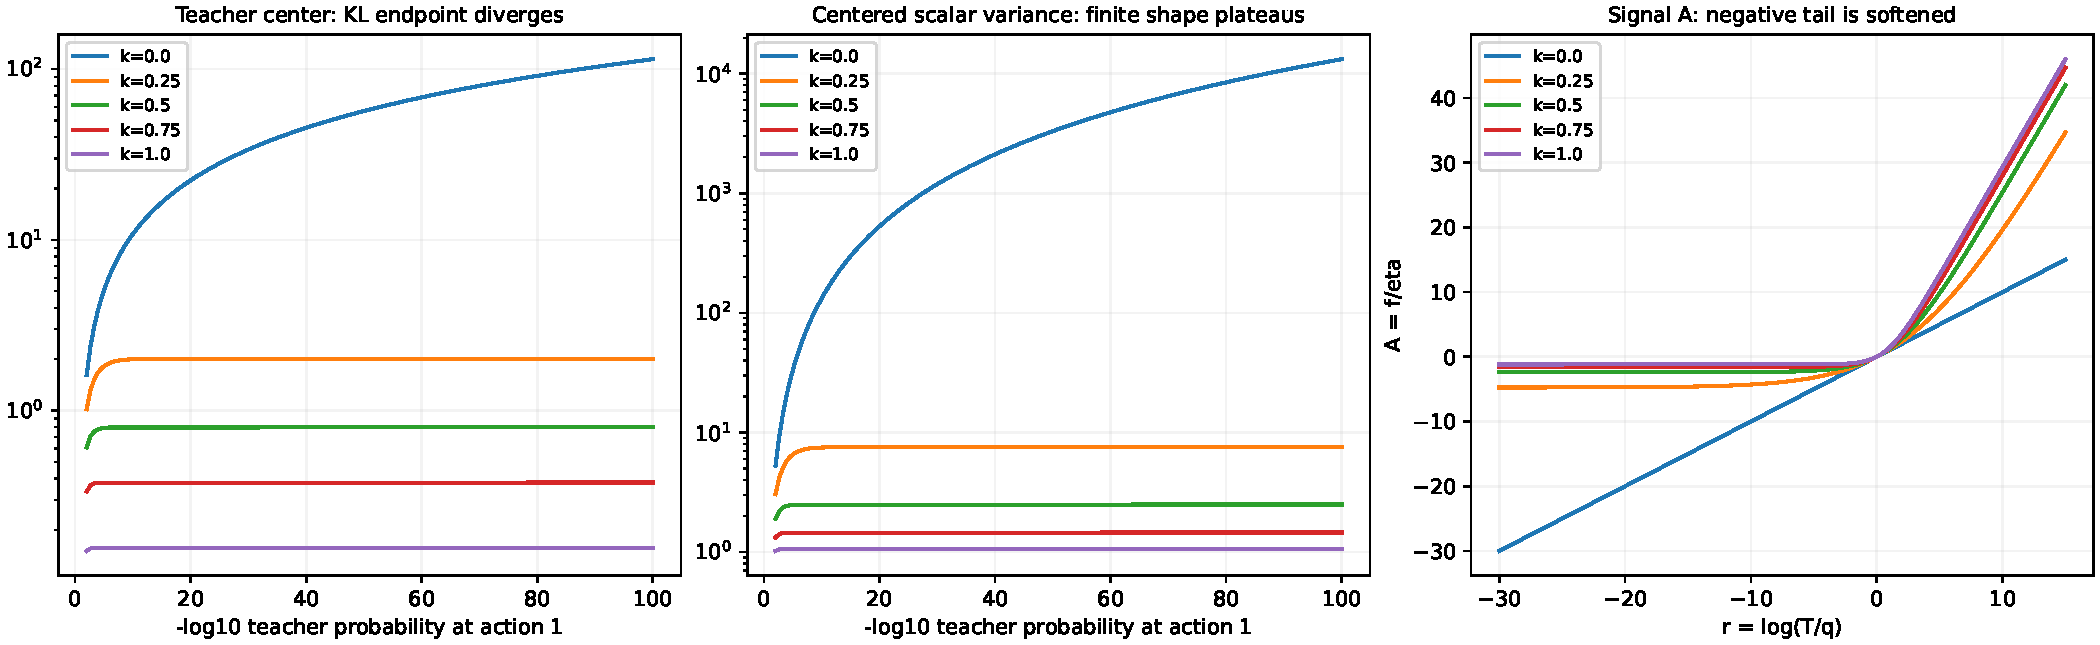
\includegraphics[width=\textwidth]{../../results/power-center-advantage/negative-tail-center-variance.pdf}
 \caption{固定 $q=(1/2,1/2)$、$\eta=0.3$，teacher 一个概率趋零时，几何中心及 advantage 方差发散，正形状出现平台。右图显示规范化信号 $A$ 的负尾部变化。曲线由完整二元分布精确求和生成。}
\end{figure}
\begin{figure}[htbp]
 \centering
 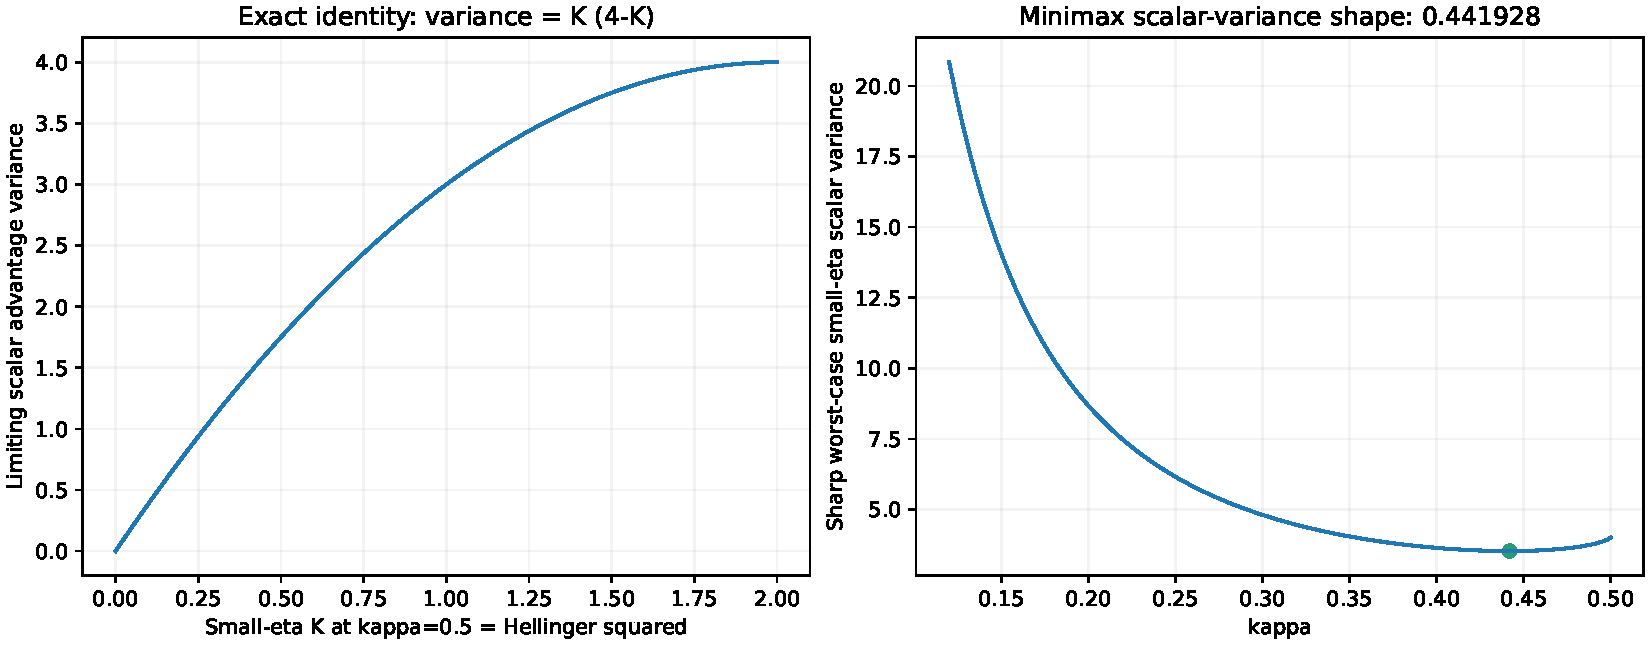
\includegraphics[width=\textwidth]{../../results/power-center-advantage/sharp-small-step-center-variance.pdf}
 \caption{左：平方根的小步极限满足 $V=K(4-K)$。右：最坏标量 advantage 方差的锐小步常数与前文自然速度常数一致，最优形状约为 $0.441928$。}
\end{figure}

\subsubsection{精确求和、Monte Carlo 与非负估计的代价}

若 teacher forward 能提供该前缀完整 logits，则使用完整 $q$ 权重直接求式~\eqref{eq:center-expanded-k}，不需要生成第二条 response。信号在 log 空间用 logaddexp 计算，避免先形成极大的 $T/q$。该中心可以按 prefix 缓存并冻结。

若采用独立 $a_i\sim q(\cdot\mid s)$，有无偏估计
\begin{equation}
 \widehat K=-\frac1M\sum_{i=1}^MA(a_i),\qquad
 \Var\widehat K=V/M.
\end{equation}
$\widehat K$ 单次可以为负；这不违背其非负期望。另一个逐样本非负无偏估计为
\begin{equation}
 \widehat K_+=\frac1M\sum_i[\rho(a_i)-1-A(a_i)].
\end{equation}
两者期望相同，方差一般不同。 它们在局部与最坏尾部上具有不同表现。若 $\rho=1+\epsilon h$、$\E_qh=0$ 且 $h$ 有界，令 $c_0=1-\kappa(1-\eta)$，则
\begin{align}
 -A&=-\epsilon h+\tfrac12c_0\epsilon^2h^2+O(\epsilon^3),\\
 \phi(\rho)&=\tfrac12c_0\epsilon^2h^2+O(\epsilon^3),\\
 \Var(-A)&=\epsilon^2\E_qh^2+O(\epsilon^3),\\
 \Var\phi(\rho)&=\tfrac14c_0^2\epsilon^4\Var_q(h^2)+O(\epsilon^5).
\end{align}
因此包括 $\kappa=0$ 在内，接近同分布时非负控制变量估计可把方差从二阶降至四阶；这需要概率比一致接近一，不能扩展到任意重尾输入。

取 $q=(\epsilon,1-\epsilon)$、$T=(1/2,1/2)$、固定 $\kappa>0,\eta<1$，原始估计方差按 $O(\epsilon\log^2(1/\epsilon))\to0$；非负估计的稀有项为 $\rho\sim1/(2\epsilon)$，其方差按 $1/(4\epsilon)$ 发散。这个 $\rho-1$ 控制变量保证非负性，却不能提供统一低方差保证。固定数据上也可能降低方差，应记录真实条件矩后判断。 即便原 KL 很小，也不能自动使用局部结论：取 $q=(\epsilon,1-\epsilon)$、$T=(\epsilon^{1/4},1-\epsilon^{1/4})$，有 $\KL(q\Vert T)\sim\epsilon^{1/4}\to0$，但非负估计的方差按 $\epsilon^{-1/2}$ 发散。概率比一致接近一比 KL 小更强。

如果独立中心估计与当前 action 独立，$\Var[A(a)+\widehat K]=V+V/M$。估计中心不会自动降低标量 advantage 方差。若中心与 advantage 使用同一组 $M$ 个 action，固定参数下
\begin{equation}
 \E\left[\frac1M\sum_i(A_i-\bar A)\psi_i\right]
 =\frac{M-1}{M}\operatorname{Cov}_q(A,\psi).
\end{equation}
这个恒等式由展开双重和得到：$M$ 个同索引项贡献 $\E A\psi$，$M(M-1)$ 个异索引项贡献 $\E A\E\psi$。$M=1$ 时更新为零。 若同一个 action 改用非负估计 $\widehat K_+=\rho-1-A$，则
\begin{equation}
 A(a)+\widehat K_+(a)=\rho_a-1,
\end{equation}
完全消掉 $\kappa,\eta$ 的教师信号形状。在 $p=q$ 时，该 score 更新的期望是 $\E_T\psi_q$，对应 forward-KL 的下降方向，而不是原 $\E_qB\psi_q$。中心估计本身无偏，不代表与当前 action 共享样本后的梯度无偏。

$M>1$ 可以使用独立中心、leave-one-out 或无偏样本协方差系数；它们要求同一 prefix 下的独立动作，不能用不同前缀的 token 直接代替。本研究的主 BPO 路线采用完整条件求和，不引入 response 组。

\subsubsection{有界非负无偏中心估计器}

$q$ 提案下的非负估计会出现重尾，但可以利用已有 $K$ 上界构造另一个提案。令 $\kappa>0,\eta<1$，$c=-\log(1-\eta)/(\kappa\eta)\ge1$。由 $A\ge-c$ 与 $\phi\ge0$，逐 action 有
\begin{equation}
 0\le q_a\phi(\rho_a)\le T_a+(c-1)q_a.
\end{equation}
右侧的总质量是 $c$，所以定义归一化包络提案
\begin{equation}
 \mu_c=(1-1/c)q+(1/c)T,\qquad
 Z(a)=\frac{q_a}{\mu_c(a)}\phi(\rho_a),\quad a\sim\mu_c.
 \label{eq:center-bounded-mixture-estimator}
\end{equation}
无需知道真实 $K$ 即可采样：以概率 $1/c$ 从教师抽一个 action，否则从锚点抽一个 action。它只估计本 prefix 的中心，不把 response rollout 改为这个提案，也不引入 response 组。

\begin{theorem}[中心估计的最小统一样本上界]
\label{thm:center-bounded-estimator}
上述估计器满足
\begin{equation}
 \E_{\mu_c}Z=K,\qquad0\le Z\le c,\qquad
 \Var_{\mu_c}Z\le K(c-K)\le c^2/4.
\end{equation}
对 $M$ 次独立抽样，$\widehat K_\mu=M^{-1}\sum_iZ_i$ 无偏、非负且不超过 $c$，其方差不超过 $K(c-K)/M$。所有分布上统一成立的无偏估计器样本上界不可能小于 $c$。
\end{theorem}

\begin{proof}
定义给出 $\E_\mu Z=\sum_aq_a\phi(\rho_a)=K$。包络不等式给出 $0\le Z\le c$，于是 $Z^2\le cZ$，取期望再减 $K^2$ 得到方差界。独立平均将方差除以 $M$。若任意无偏估计器总被常数 $b$ 上界约束，则 $K=\E\widehat K\le b$；而前面的正支持见证可以使 $K\to c$，故 $b\ge c$。这个最优性只作用于统一样本上界，不宣称该提案在每个固定分布上具有最小方差。\hfill$\square$
\end{proof}

Hoeffding 不等式还给出明确的置信界
\begin{equation}
 \Pr\{ |\widehat K_\mu-K|\ge\epsilon\}
 \le2\exp(-2M\epsilon^2/c^2).
\end{equation}
$\kappa=0$ 或 $\eta=1$ 的 KL 在分布类上无界，因此不能保持一个有限统一样本上界的无偏估计器。固定已知分布可以有有限界，不能与这个分布类结论混同。

平方根的小步极限尤为直观：$c\to2$、$\mu_c\to(q+T)/2$、$\phi(\rho)\to(\sqrt\rho-1)^2$，于是
\begin{equation}
 Z_0(a)=\frac{2(\sqrt{T_a}-\sqrt{q_a})^2}{T_a+q_a}\in[0,2],
 \qquad\E_{(q+T)/2}Z_0=H^2(q,T).
\end{equation}
记 $K_{\mathrm H}=H^2$，则 $\Var Z_0\le K_{\mathrm H}(2-K_{\mathrm H})$；而 $q$ 提案下的原始有符号中心估计在此极限具有方差 $K_{\mathrm H}(4-K_{\mathrm H})$。因此在每个固定完整支持分布对的平方根小步极限，包络估计方差至多为原始估计的一半。有限 $\eta$ 时不保证逐输入都优于原始有符号估计，真实条件矩仍需报告。 若当前 $q$ action 与 $M$ 个中心样本独立，则估计 advantage $\widehat B=A(a)+\widehat K_\mu$ 的方差为 $V+\Var Z/M$。平方根小步极限因此满足
\begin{align}
 \Var\widehat B
 &\le K_{\mathrm H}(4-K_{\mathrm H})
    +K_{\mathrm H}(2-K_{\mathrm H})/M\\
 &\le4+\frac1{M(M+1)}.
\end{align}
第二步在 $K_{\mathrm H}\in[0,2]$ 上最大化该凹二次式，驻点为 $(2M+1)/(M+1)$。一个独立辅助中心 action 即 $M=1$ 时，上界为 4.5；使用有符号 $q$ 中心估计的对应统一界为 8。这个结论作用于冻结 prefix 的教师标量 advantage，并要求独立性；它不涵盖学生反馈项或直接成为全参数梯度方差定理。


主 BPO 的完整条件求和无需这个辅助估计器。若使用它构造 sampled-action advantage，中心抽样仍须与当前 action 独立，或者给出相关性修正；有界中心估计不使 $A$ 的正尾部变为有界，也不自动解决整段 inner 的缓存误差。单样本中心只需本前缀辅助 action，不能把它解释为新增完整 response。

\subsubsection{有限 head 与尾部质量的中心区间}

令 $S$ 为任一保留 head，$\delta=\sum_{a\notin S}q_a$、$\tau_T=\sum_{a\notin S}T_a$，记 $K_S=-\sum_{a\in S}q_aA_a$。当 $\delta>0$，尾部的 $\rho$ 条件均值为 $\tau_T/\delta$。函数 $-A(\rho)$ 凸且不超过 $c$，由 Jensen 得到
\begin{equation}
 \boxed{K_S-\delta A(\tau_T/\delta)
 \le K\le K_S+\delta c_{\kappa,\eta}.}
 \label{eq:center-head-tail-interval}
\end{equation}
下界正是把尾部合并为一个 action 后的中心，亦为对应 $f$-divergence 的数据处理下界。区间宽度为 $\delta[c+A(\tau_T/\delta)]$，可直接计算；$\delta=0$ 时直接用完整 head 和。几何端点仍有 Jensen 下界，但没有仅靠两种尾部质量获得的有限统一上界。 对嵌套 head，拆分尾部由 Jensen 保证下界非减少；新增 action $a$ 对上界的改变量为 $q_a[-A_a-c]\le0$，所以上界非增加。可以持续扩大 head，直到区间宽度不超过 $\epsilon$，再取中点获得绝对中心误差不超过 $\epsilon/2$ 的确定性证书。

以一个已估计中心代替精确 $K$，会给 BPO score 系数加入常数误差 $\Delta K$。若 $\Delta K=\widehat K-K$，当前学生不等于 $q$ 时，梯度偏差为 $-\Delta K\E_q\psi_p$，若 $\|\psi_p\|\le M$，其范数不超过 $M|\Delta K|$。因此区间既报告中心误差，也能给固定参数下的 score 偏差提供证书。 这个偏差结论作用于停止系数并使用原始 $\psi_p$ 的 score 更新。若精确微分学生条件中心，情况不同：固定的教师中心误差使完整平方损失仅增加 $\eta(\Delta K)^2/2$，不改变其梯度。对应无偏形式是
\begin{equation}
 g_{\mathrm{cscore}}=
 [C_qU/\eta-A-\widehat K]\,[\psi_p-\E_q\psi_p].
\end{equation}
对于固定参数、精确学生中心和不依赖当前 action 的任意冻结 $\widehat K$，其 $q$ 期望等于真实 BPO 梯度。也可以通过停止系数乘以 $\log p(a)-\E_q\log p$ 实现这个梯度；教师中心于是只影响该估计器的方差；若其误差不消失，在 $p=m$ 处仍可能保留采样噪声，不能自动继承精确残差估计器的零噪声性质。若中心来自当前 action，或学生中心也只是有偏近似，则不能直接套用这项结论。


\subsubsection{标量中心不等于最优梯度 baseline}

在 inner 起点 $p=q$，$\E_q\psi_q=0$，任意常数 baseline 都保持教师 score 梯度期望。令 $w(a)=\|\psi_q(a)\|^2$，则使协方差 trace 最小的 baseline 为
\begin{equation}
 b_\star=\frac{\E_q[A w]}{\E_qw},\qquad
 V_g(b)=\E_q[(A-b)^2w]-\|\E_qA\psi_q\|^2.
\end{equation}
配方平方给出
\begin{equation}
 V_g(\E_qA)-V_g(b_\star)
 =\E_qw\,(\E_qA-b_\star)^2\ge0.
\end{equation}
因此精确均值中心 $-K$ 不保证梯度方差最小，也不保证优于不使用 baseline。二元 $q=(0.99,0.01)$、$T=(0.5,0.5)$、$\kappa=0.5$、$\eta=0.3$ 下，categorical logit 梯度协方差 trace 从无 baseline 的 0.92622 增至均值 baseline 的 1.07537，而 score 加权最优 baseline 在这个二元例子中给出零方差。

当前 $p\ne q$ 时，$\E_q\psi_p$ 通常非零，不能直接替换 BPO 中心而保持梯度不变。若需要额外调整 residual baseline，须加入相应确定性补偿项。教师 $K$ 是 BPO 目标定义的一部分，最优 score baseline 是估计器的另一个选择。

教师 advantage 的性质主要控制 inner 起点。一般 inner 的净监督是 $B-C_qU/\eta$；学生反馈可能无界。前节的残差二阶矩界 $\E\|g\|^2\le(2M^2/\eta)\mathcal L_{\mathrm{BPO}}$ 仍适用，但不把教师单侧界升级为全训练系数的绝对界。

\begin{figure}[htbp]
 \centering
 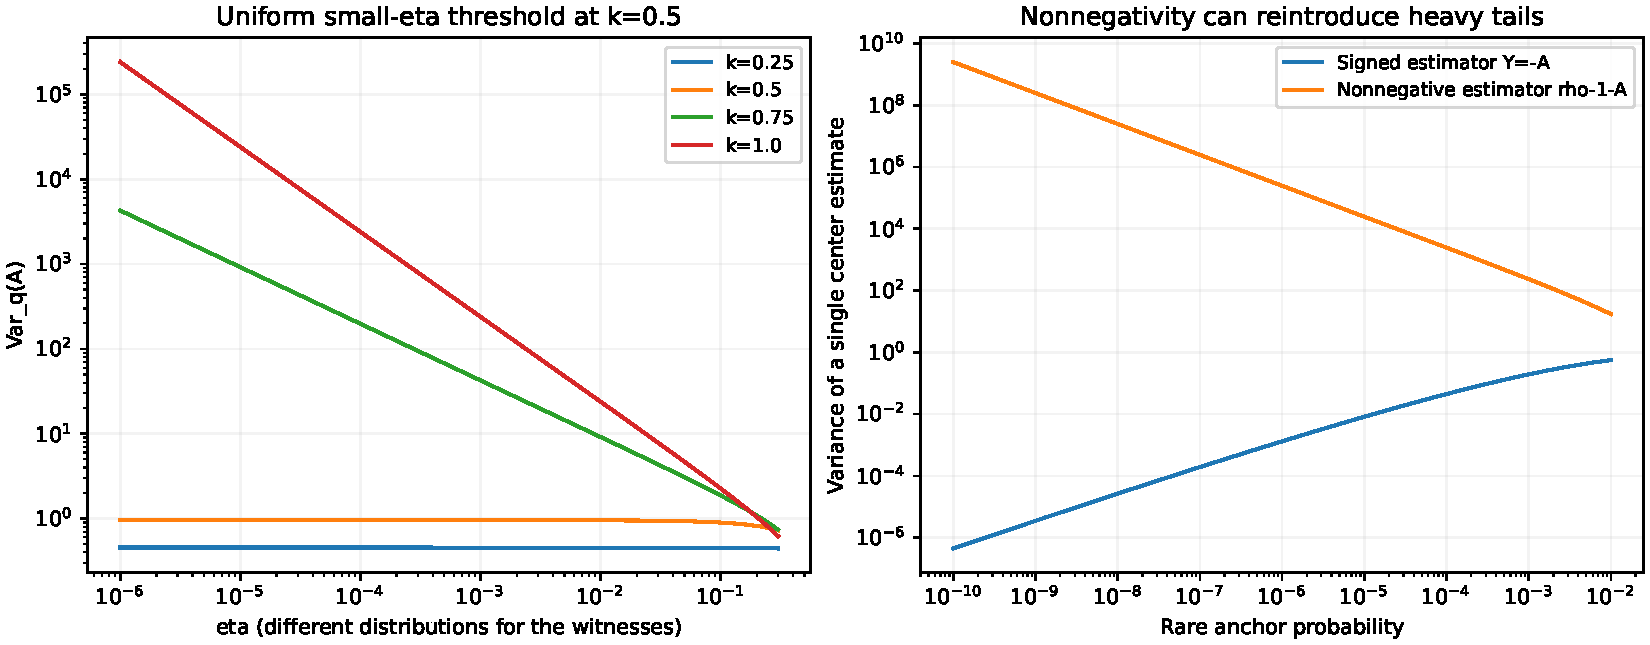
\includegraphics[width=\textwidth]{../../results/power-center-advantage/small-step-and-estimation.pdf}
 \caption{左：小步方差阈值的下界见证，不同形状使用不同分布族，不能当作同数据上的性能排名。右：逐样本非负中心估计可能重新引入概率比重尾。}
\end{figure}
\begin{figure}[htbp]
 \centering
 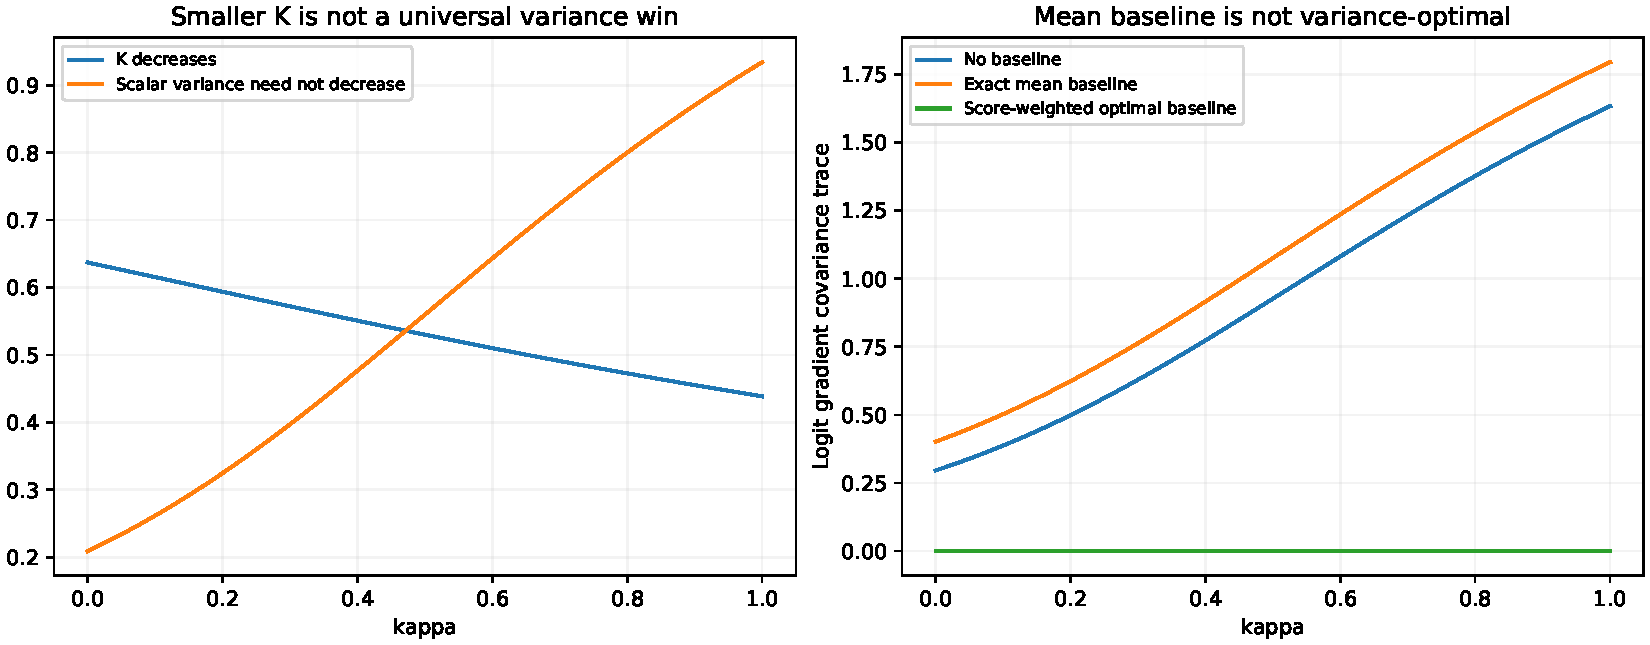
\includegraphics[width=\textwidth]{../../results/power-center-advantage/baseline-counterexample.pdf}
 \caption{同一二元输入下，$K$ 随形状下降但标量方差不必下降；均值 baseline 也不一定降低 logit 梯度方差。零方差最优 baseline 是二元例子的性质，不是一般网络结论。}
\end{figure}

数学核验与真实缓存审计见 \path{experiments/analysis/power_center_advantage.py}；真实缓存取原 64 条 t22 response 每条两个固定随机 reservoir 位置，共 128 个 prefix，对 20 组 $\kappa,\eta$ 精确求 action 条件矩。结果与所有实验统一维护在唯一实验报告；这些 CPU 模型分布统计不等于新 GPU 训练或全参数梯度方差。
